\chapter{Design}

The Design chapter talks about the architectural blueprint of VitalMonitor. This includes an overview of the system's architecture, followed by an in-depth analysis of each component's design and role within the larger ecosystem. From the setting up of the database to the intricate firmware running on each smart patch, the design choices made across VitalMonitor will be explored to elucidate their contributions to the system's overall functionality, reliability, and scalability. This chapter is written in accordance with v8 iteration of the firmware.\\

Additionally, the chapter illustrates the thoughtful considerations behind the chosen architectural patterns, dissects the interactions between system components, and explains the rationale behind the design decisions. This chapter sets the stage for understanding how each element of VitalMonitor contributes to a cohesive and robust system.

\section{System Design}
\subsection{Design Approach}

\noindent The system design of VitalMonitor integrates multiple architectural principles, deviating from traditional approaches to create a tailored solution. It is structured into three primary layers: Presentation, Application, and Data Layer.

\begin{itemize}
    \item \textbf{Presentation Layer:}  The web dashboard serves as the presentation layer, providing a user interface (UI) for users to interact with the system. This layer presents data collected from IoT devices in a visual and understandable format through the dashboard.
    
    \item \textbf{Application Layer:} The middleware component serves as the application layer, handling the business logic of receiving, and distributing data from Smart Patches. It acts as an intermediary between the presentation layer and the data layer, performing tasks such as data aggregation and routing.
    
    \item \textbf{Data Layer:} The Smart Patches represent the data layer, where data is generated and collected from the real world. This raw data from sensors is then processed and transmitted to the middleware for further processing and storage.

    
\end{itemize}
Communication between these layers primarily occurs through APIs, designed following RESTful principles to promote simplicity and flexibility. \\ \\
Moreover, the Smart Patch logic adopts a hybrid architecture:
\begin{itemize}
    \item \textbf{Edge-Computing:} Edge Computing optimizes data processing by executing computations closer to the data source (here the Smart Patch), effectively reducing latency and conserving bandwidth. This strategy facilitates local data processing, eliminating irrelevant information and transmitting only essential insights to the cloud.  Urgent actions, like sending emergency SMS via Twilio API, are executed swiftly at the edge to minimize delays.
    
    \item \textbf{Cloud-Based:} The cloud serves dual purposes: firstly, as a data repository, and secondly, for processing incoming data from devices. Settings originating from the Presentation layer are forwarded to Smart Patches from the cloud.

\end{itemize}

\noindent This design rationale was chosen to:
\begin{enumerate}
\item Enhance flexibility in development and deployment processes.
\item Facilitate continuous integration and delivery practices.
\item Inherently support a distributed data processing model, crucial for IoT environments.
\end{enumerate}

\subsection{Component Roles and Ideology}

\noindent{VitalMonitor operates on a coordinated data flow mechanism, where each component plays a critical role. Each component is designed with a specific role in mind as per the above design choices. This systematic interaction ensures seamless end-to-end data flow, from data capture to user-level presentation. The components are: }

\begin{itemize}
    \item The Dashboard is the user interface through which users interact with the system. It is designed to offer intuitive controls and insightful analytics.

    \item The Smart Patch is a component of VitalMonitor, equipped with sensors and a microcontroller to accurately collect and relay vital health data.

    \item The Middleware acts as the central nervous system, directing the flow of information and ensuring the components of VitalMonitor communicate effectively.
\end{itemize}

\subsection{Data Flow Architecture}
\noindent{Figure \ref{fig:dfd-1} illustrates the interconnectivity and the specific pathways through which data travels within the VitalMonitor system. This diagram provides a visual representation of the sequential and logical flow of data, from the initial collection at the smart patch, through processing by the middleware, to its final storage and presentation in the dashboard. Figure \ref{fig:dfd-2} goes further into how a Smart Patch gets data from sensors and integrates with Twilio API and Adafruit IO. It exemplifies how the design ensures not only the efficient management of data but also its security and integrity as it moves through various system components.}

\begin{figure}[h!]
    \centering
    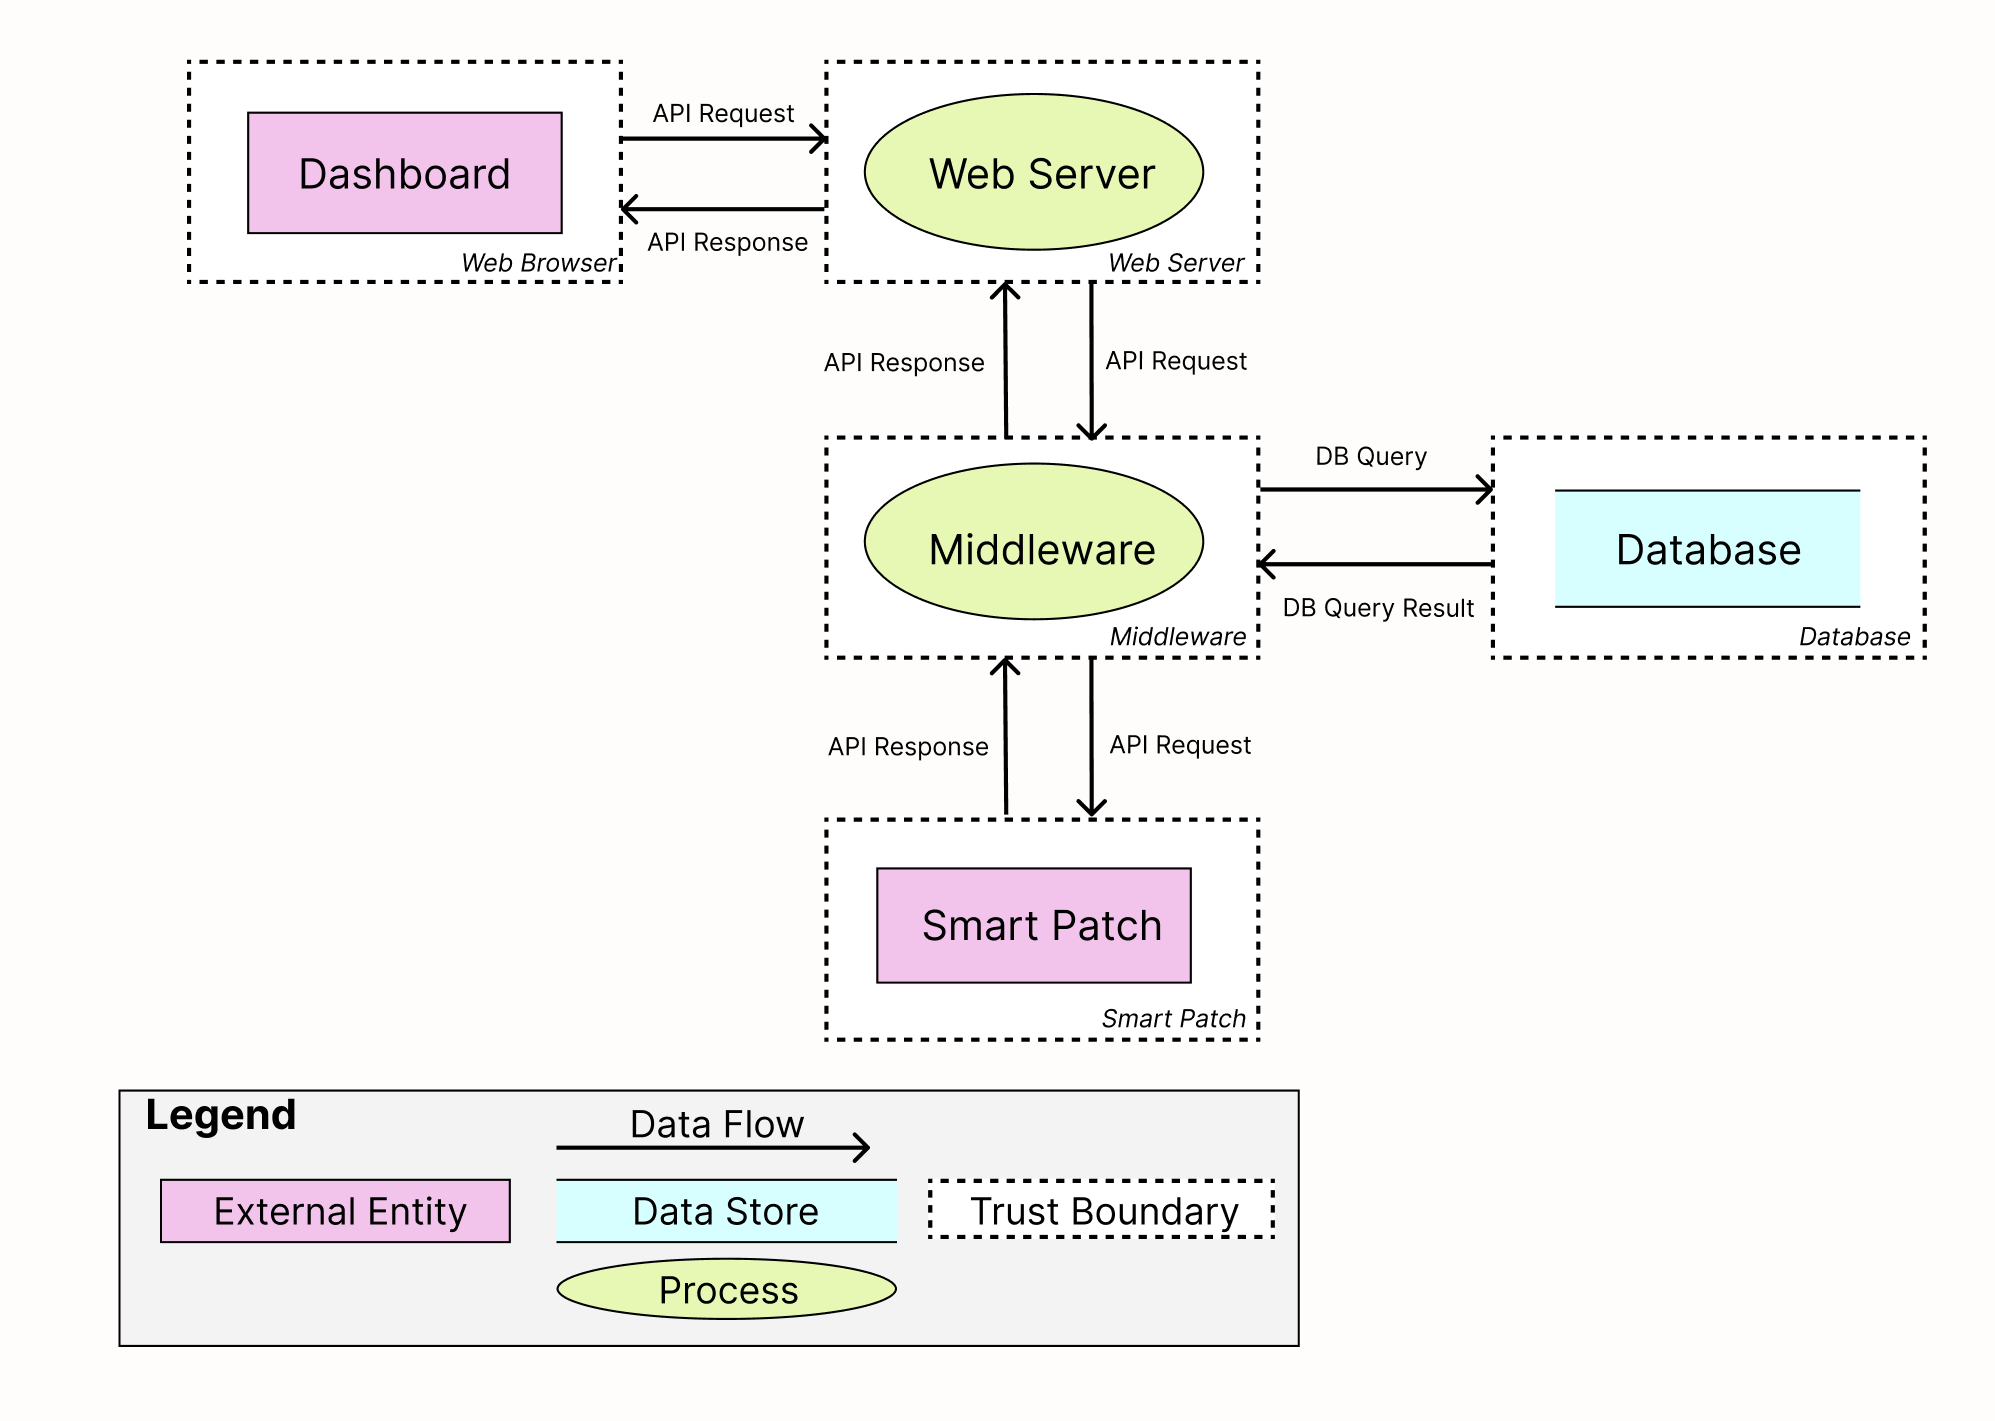
\includegraphics[width=1\linewidth]{images/system-design-data-flow-full.png}
    \caption{Data Flow Diagram 1}
    \label{fig:dfd-1}
\end{figure}

\begin{figure}[h!]
    \centering
    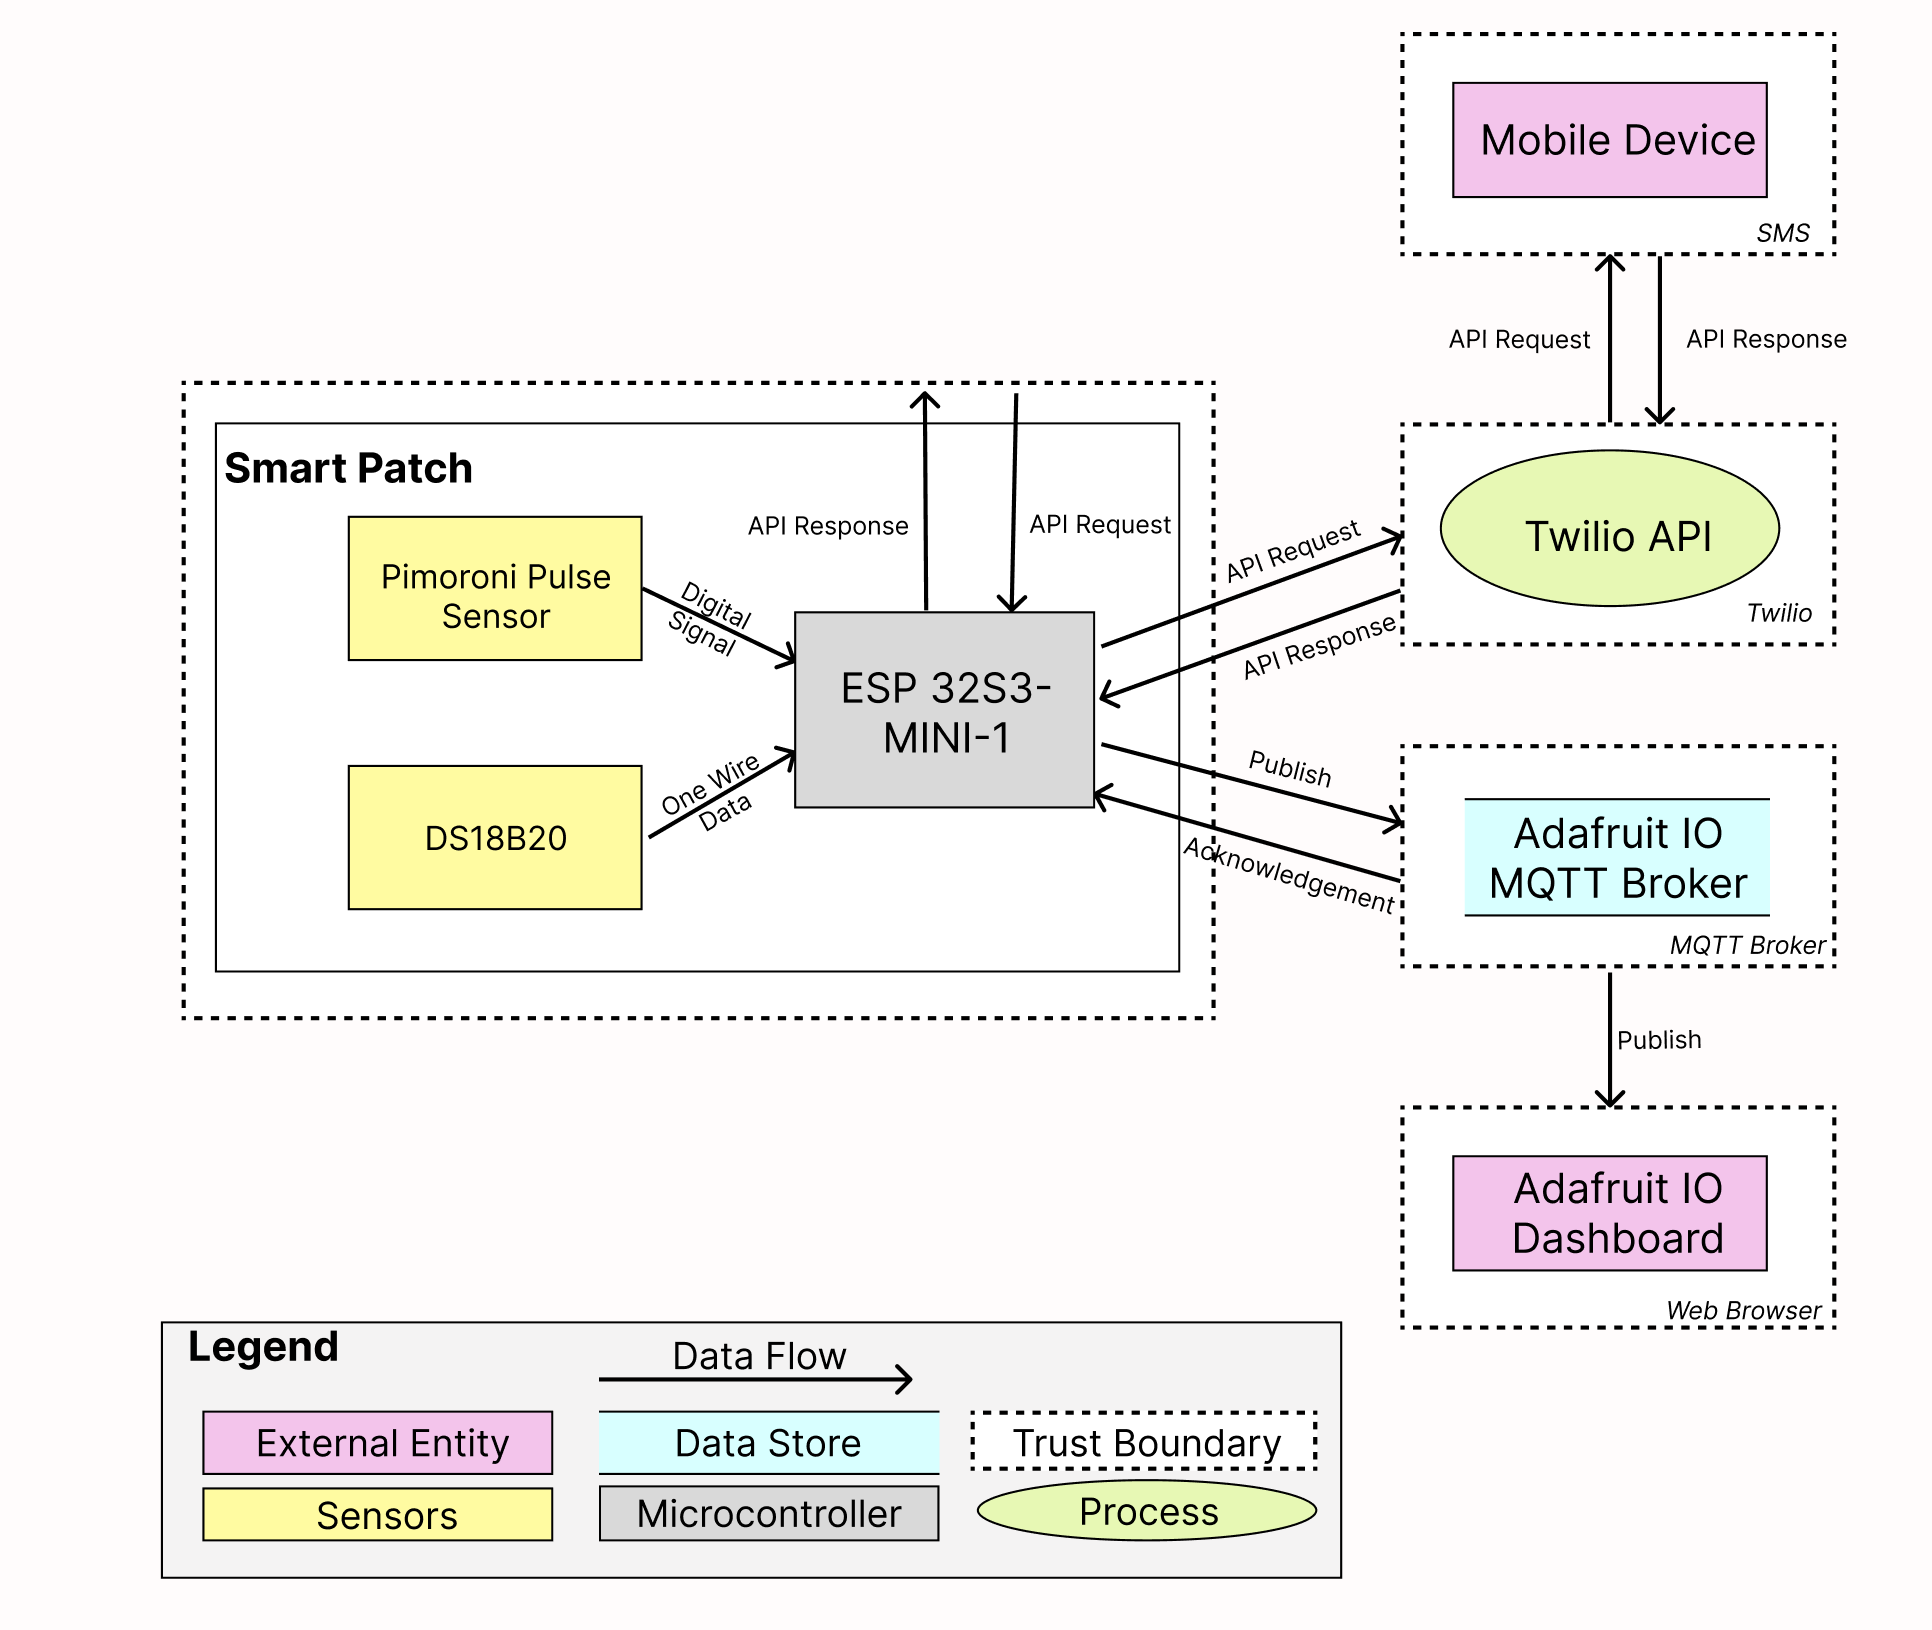
\includegraphics[width=1\linewidth]{images/system-design-data-flow-smart-patch.png}
    \caption{Data Flow Diagram 2}
    \label{fig:dfd-2}
\end{figure}


\newpage
\section{Database Design}
The database is designed using MySQL and is hosted on Google Cloud, leveraging the platform's scalable infrastructure to handle the data management needs of the IoT ecosystem. With a focus on relational integrity and query efficiency, the database schema is structured to support the platform's core functionalities: user management, device tracking, and real-time data analytics.\\

\noindent Figure \ref{fig:database-diagram} provides a visual representation of the relational models and their interconnections. It illustrates the foreign key relationships and cardinality between tables, reflecting the database's normalized design that promotes data integrity and reduces redundancy.\\ \\ \\ 

\begin{figure}[!h]
    \centering
    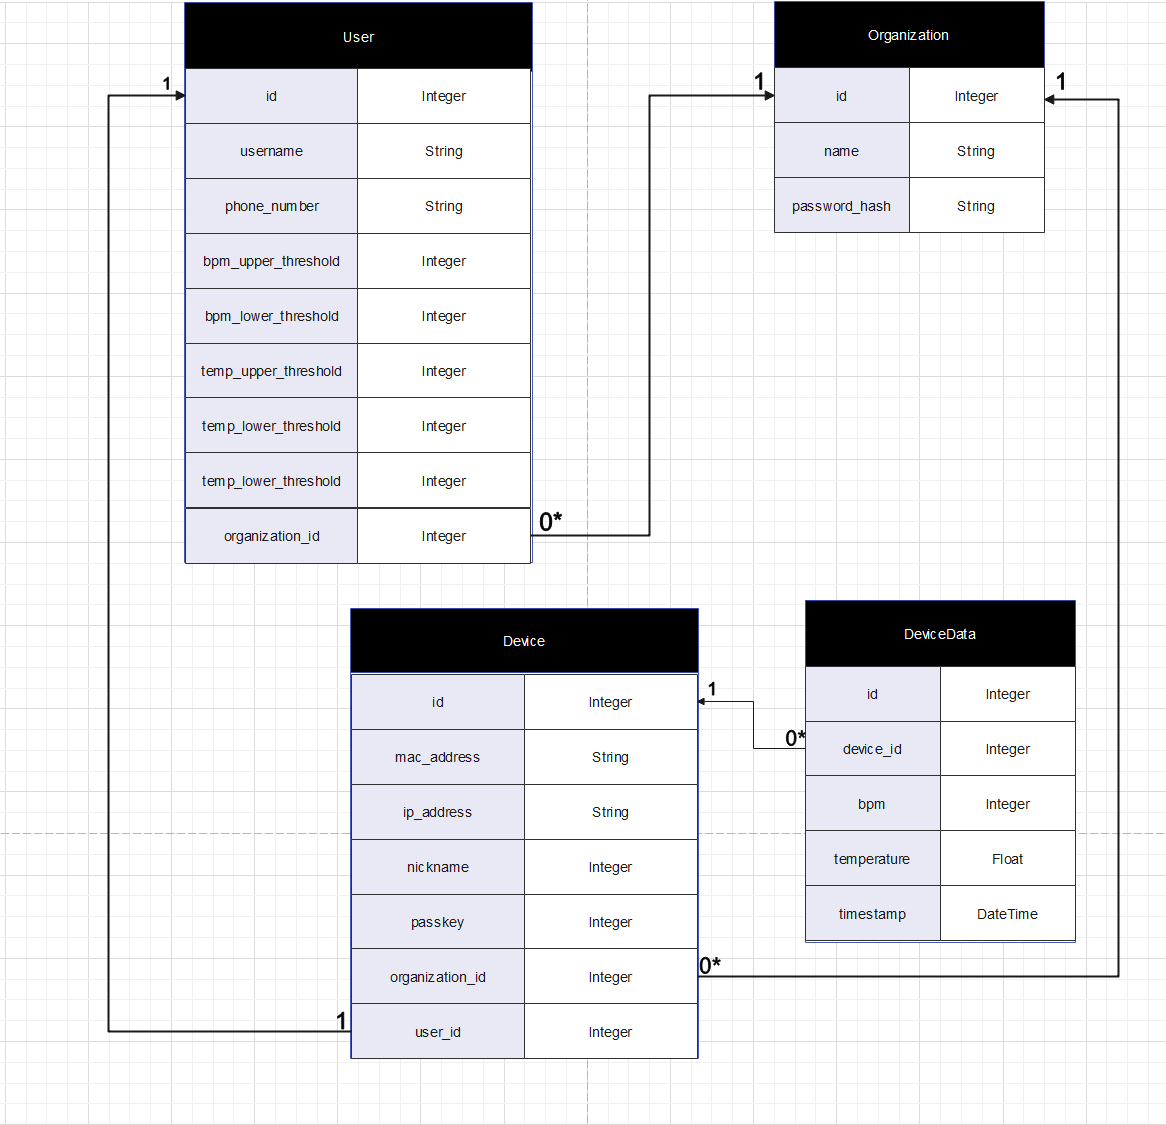
\includegraphics[width=\linewidth]{images/database-obj-relation.png}
    \caption{Database Diagram}
    \label{fig:database-diagram}
\end{figure}

\noindent The main entities of the database are:
\subsection{Organizations}
Organizations form the top hierarchical level within VitalMonitor, representing entities that manage a collection of users and devices. The organization's model features fields for identification, authentication, and relationships to devices and users. Robust security measures are implemented, including hashed passwords using bcrypt to safeguard access credentials.

\subsection{Devices}
The Device model is a representation of physical IoT devices in the system, uniquely identified by a MAC address. Devices are associated with an organization and optionally linked to a specific user. Each device holds a passkey for secure communications and maintains a record of health data streams through its one-to-many relationship with the DeviceData model.

\subsection{Users}
Users are associated with an organization and have a direct connection to a single device. The User model contains contact information and configurable thresholds for health metrics, enabling personalized monitoring and alerts.

\subsection{DeviceData}
The DeviceData model captures the essence of IoT functionality within VitalMonitor. It stores time-series data from IoT devices, including heart rate (bpm) and temperature readings, with precise timestamps. This model ensures that vital health data is recorded, enabling historical data analysis and real-time monitoring.\\

\noindent The database's design is crafted to be intuitive and efficient, facilitating straightforward interactions for the system's backend services. By adopting this structured approach, VitalMonitor ensures fast retrieval of data, which is paramount for real-time applications, while also maintaining the flexibility to scale and adapt to future requirements. \\

\noindent The firmware is designed to handle the exchange of threshold parameters and user information with the middleware. If the measured bpm or temperature exceeds the set thresholds, the device utilizes the Twilio API to dispatch an SMS to a designated emergency contact.

\section{Smart Patch (Firmware) Design}

The firmware for Smart Patch is an ESP32S3-MINI-1 microcontroller. It constitutes the operational bedrock for interfacing with the hardware sensors and executing the device's logic. It is meticulously programmed to manage sensor data acquisition, device control, network communication, and emergency alerting functionalities.

\subsection{Hardware Components}
The device is equipped with a DS18B20 temperature sensor and a Pimoroni Pulse Sensor, tasked with measuring the user's body temperature and heart rate, respectively. The temperature sensor circuit includes a 4.3k\(\Omega\) pull-up resistor essential for accurate signal readings. Similarly, a 1k\(\Omega\) resistor is employed in the LED circuit to indicate the device's operational status. Activation of the sensors and publication of data is controlled by a user-operated push button which toggles the data transmission process, with an LED serving as a visual indicator for the current state—lit when data is being sent and unlit otherwise. The device is powered by a LiPo battery, ensuring portability and convenience.


\subsection{Hardware Circuit Diagram}
A detailed circuit diagram is shown in figure \ref{fig:full-circuit-diagram} outlines the wiring and connections of all components. This showcases the precise electrical relationships and configurations necessary for optimal performance. This diagram serves as a guide for the physical assembly of the hardware components. In the diagram 3V connection is shown using a red wire and ground (or GND) connection is shown using a blue wire. Legend to this figure is provided in figure \ref{fig:legend-circuit}. \\ \\
\begin{figure}[h!]
    \centering
    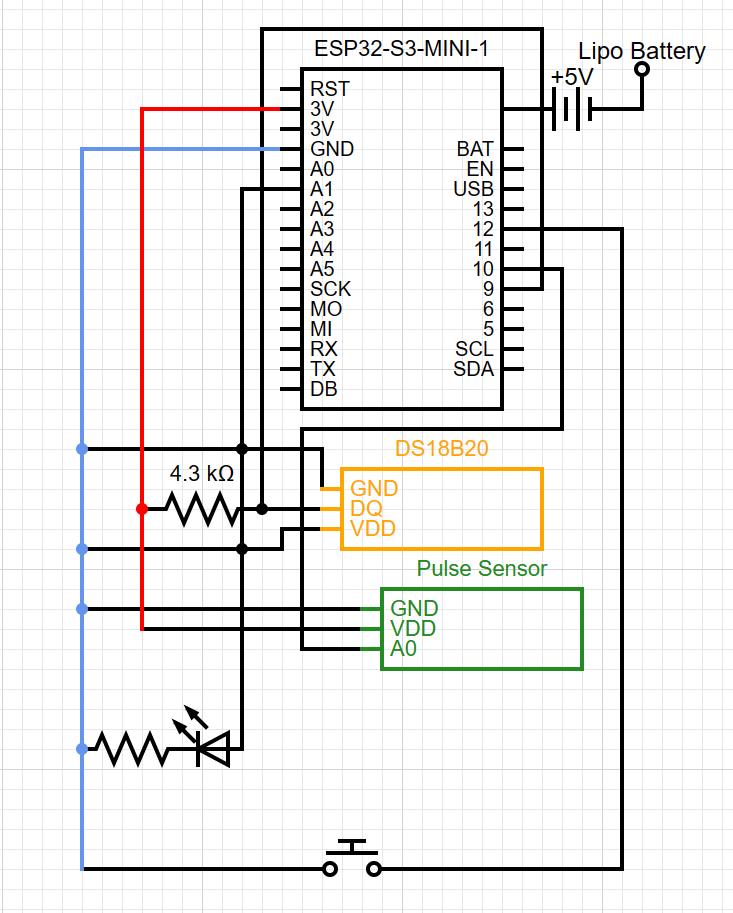
\includegraphics[width=0.8\linewidth]{images/full-circuit-diagram-2.png}
    \caption{Circuit Diagram of Smart Patch}
    \label{fig:full-circuit-diagram}
\end{figure}
\begin{figure}[h!]
    \centering
    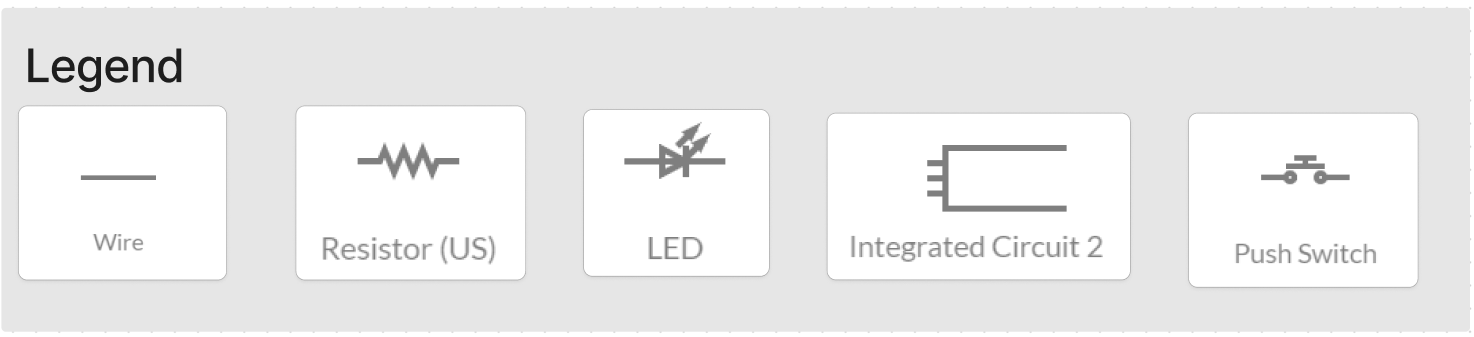
\includegraphics[width=1\linewidth]{images/legend-circuit.png}
    \caption{Legend for circuit diagram}
    \label{fig:legend-circuit}
\end{figure}

\noindent Adafruit IO Dashboard is also designed to get data directly from the firmware for testing purposes. This dashboard allows lightweight transfer of data and allows visualisation (eg., time-series graph) of the health data - which is useful to see how efficiently the data is read by the sensors.  Check Appendix \ref{app:adafruit} for more details on Adafruit IO Dashboard and how it works.


\newpage
\section{Middleware Design}

The Middleware within VitalMonitor serves as the central communication hub, orchestrating interactions among the platform's components. It acts as the pivotal component that integrates dashboards, databases, and smart patches, ensuring seamless functionality and cohesion.

\begin{figure}[!h]
    \centering
    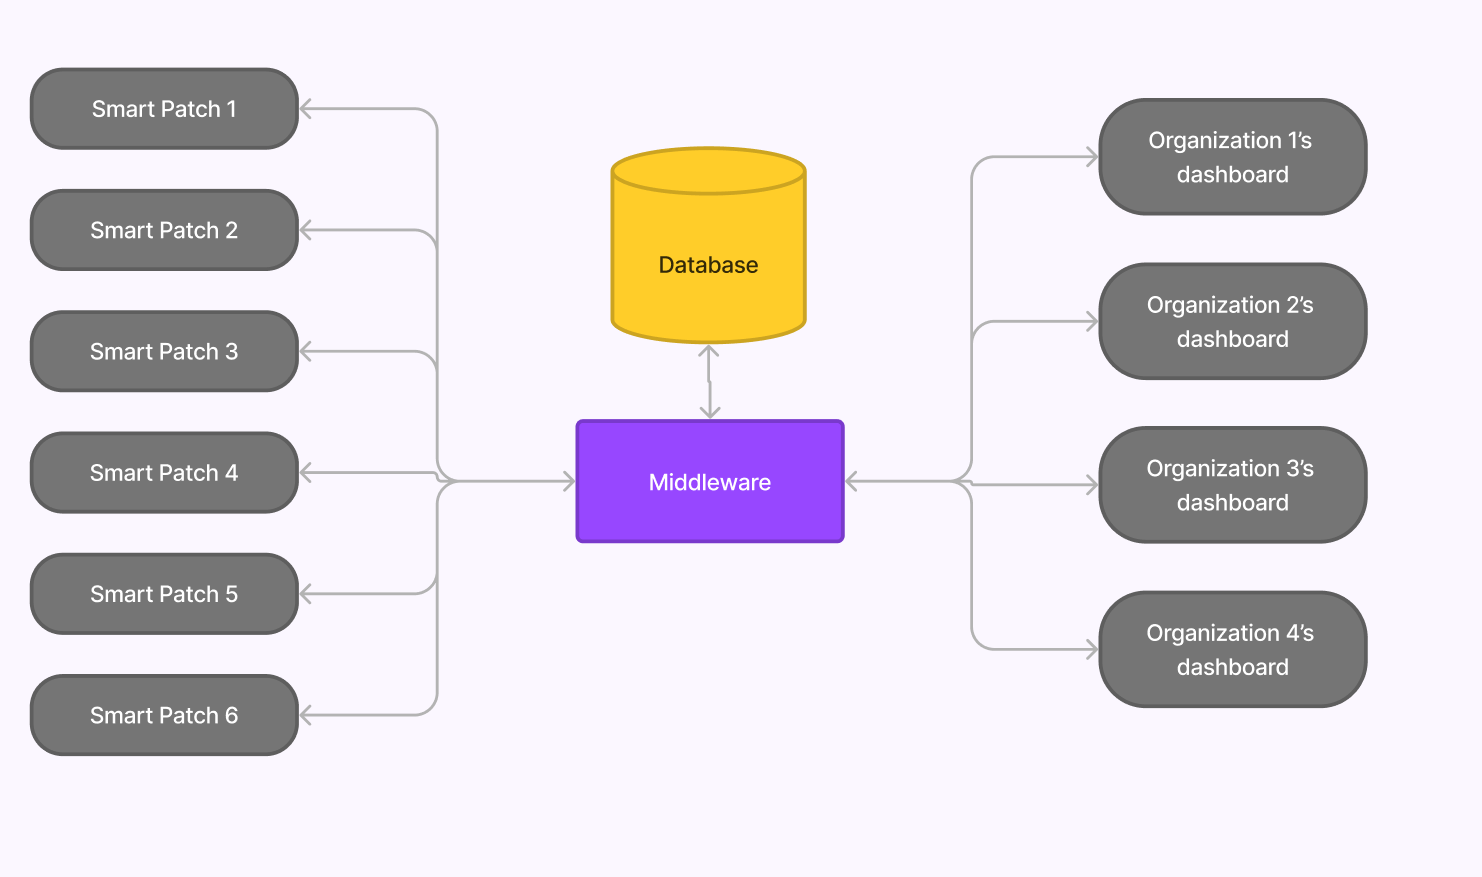
\includegraphics[width=1\linewidth]{images/compressed-data-flow.png}
    \caption{Middleware}
    \label{fig:dfd-3}
\end{figure}

\subsection{Architecture and Responsibility}
The Middleware, designed as an Application Server Middleware (ASM), bears the responsibility of overseeing vital functions necessary for the optimal operation of the VitalMonitor platform. It shoulders tasks such as processing requests, enforcing business logic, managing data, and facilitating communication between the different components of the system.\\

\noindent Additionally, following a microservices-like architecture, the Middleware offers four primary services to the system:

\begin{itemize}
    \item Session Management Service
    \item User and Device Management Service
    \item Data Ingestion Service
    \item Data Retrieval Service
\end{itemize}

\noindent This is done in such a way because when the load of number of devices and dashboard increases, the middleware will not be able to handle it. There fore, in future, isolating the service and having them as their own services along with a load balancer, this allows more controlled and managed data. 

\subsection{Design Principles}
Several key principles guided the design of the Middleware:
\begin{enumerate}
    \item \textbf{Communication Hub:}
The Middleware is designed to be a central communication hub. It is responsible for the uninterrupted flow of data between devices and the user interface. It acts as the API Gateway, receiving API calls from the dashboard, interpreting them, and routing these to the appropriate services or data stores.
\item \textbf{Abstraction:}
The Middleware is designed to provide a level of abstraction that simplifies interactions between the user interface and the system's backend. It abstracts the complexities of the underlying database structures and device communication protocols from the end-user, presenting a simple and coherent interface to the dashboard and using of smart patch.
\item \textbf{Data Management:}
The Middleware is designed to provide robust data management. It provides a secure and efficient gateway to the database, handling transactions, query processing, and data synchronization. This ensures data integrity and consistent state across the platform, even as it scales.
\item \textbf{Unified Connection for Multiple Entities:}
The Middleware is designed with a comprehensive routing and authentication system. This facilitates concurrent connections across multiple dashboards and smart patches. It supports a multiplexed network structure where each entity is uniquely identified and managed, maintaining a coherent state across the ecosystem.
\end{enumerate}

By adhering to these principles, the Middleware embodies a pivotal component within the VitalMonitor ecosystem - fostering efficient communication, seamless operation, and scalable growth.

\section{Dashboard Design}

The VitalMonitor dashboard is specifically designed to serve as a centralized control panel for organization administrators, enabling them to efficiently manage healthcare professionals' data. This platform facilitates real-time monitoring and management of user profiles and devices, allowing admins to set health thresholds, add or delete users, and assign devices. The dashboard is crafted to cater to the specific needs of health organization administrators, providing them with intuitive tools to enhance operational efficiency and patient care.

\subsection{Technology and Tools}
The dashboard is designed using Flask, a micro web framework that offers flexibility and simplicity for server-side logic. Flask's lightweight and modular nature makes it an ideal choice for constructing a responsive and efficient web application. For the frontend, HTML, CSS, and JavaScript are employed to create a dynamic and interactive user interface that responds to the administrators' operational needs effectively.

\subsection{Design Pattern}


\subsubsection{Decorator Pattern}
The use of the Decorator Pattern is fundamental in the design of our Flask application, especially in managing route associations and enhancing function capabilities without modifying their core responsibilities:

\begin{itemize}
    \item \textbf{Routing}: Utilizing Flask's @app.route() decorator simplifies the mapping of HTTP requests to Python functions, making the association between URL routes and server-side logic clear and maintainable.
    \item \textbf{Custom Decorators}:  Custom decorators are designed to manage user session and authentication checks. These intercept and verify requests to ensure user authentication before accessing specific functionalities, thus enhancing security and user management efficiency.
\end{itemize}

\subsubsection{Model View Controller-like Structure}
While Flask does not enforce an MVC architecture, the design of the dashboard subtly incorporates elements of this pattern, enhancing clarity and separation within the application:

\begin{itemize}
    \item \textbf{Model (M)}: The business logic and data interactions are handled in the background, interfacing with the middleware. This includes user and device management functionalities, where data integrity and operations like add, update, and delete are executed. Middleware provides access to requested data but not the full model and its data directly, for an additional layer of security. 
    \item \textbf{View (V)}: The presentation layer is managed through Flask’s template system. HTML templates are rendered based on the data processed by the controllers, providing a user-friendly interface for interaction. Templates for pages like \textit{add\_device.html} and \textit{user\_page.html} define how data is presented and ensure a consistent user experience.
    \item \textbf{Controller (C)}: Flask routes act as controllers, orchestrating the application's response to user inputs and interactions. They process incoming requests, call the appropriate model functions, and determine the correct views to render, completing the user request lifecycle.
\end{itemize}

\newpage
\subsection{User Flow}
The user flow diagram (Figure \ref{fig:user-flow}) visually represents the navigational pathway administrators take through the dashboard. It highlights the sequence of interactions from login to detailed device and user management.

\begin{figure}[!h]
    \centering
    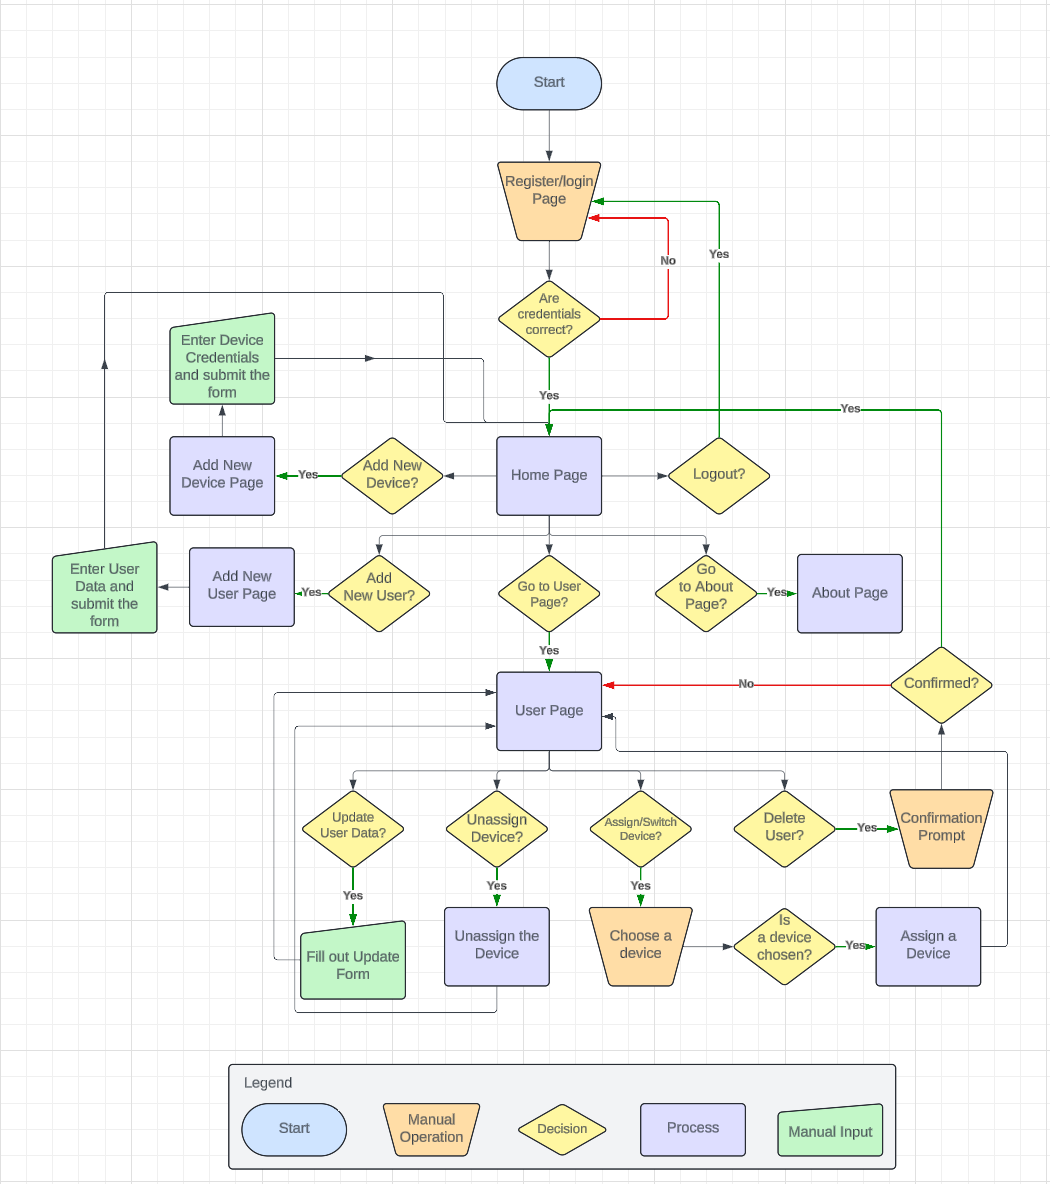
\includegraphics[width=1\linewidth]{images/user-flow.png}
    \caption{User Flow Diagram for Dashboard}
    \label{fig:user-flow}
\end{figure}

\subsection{Wireframes}
\begin{figure}[!h]
    \centering
    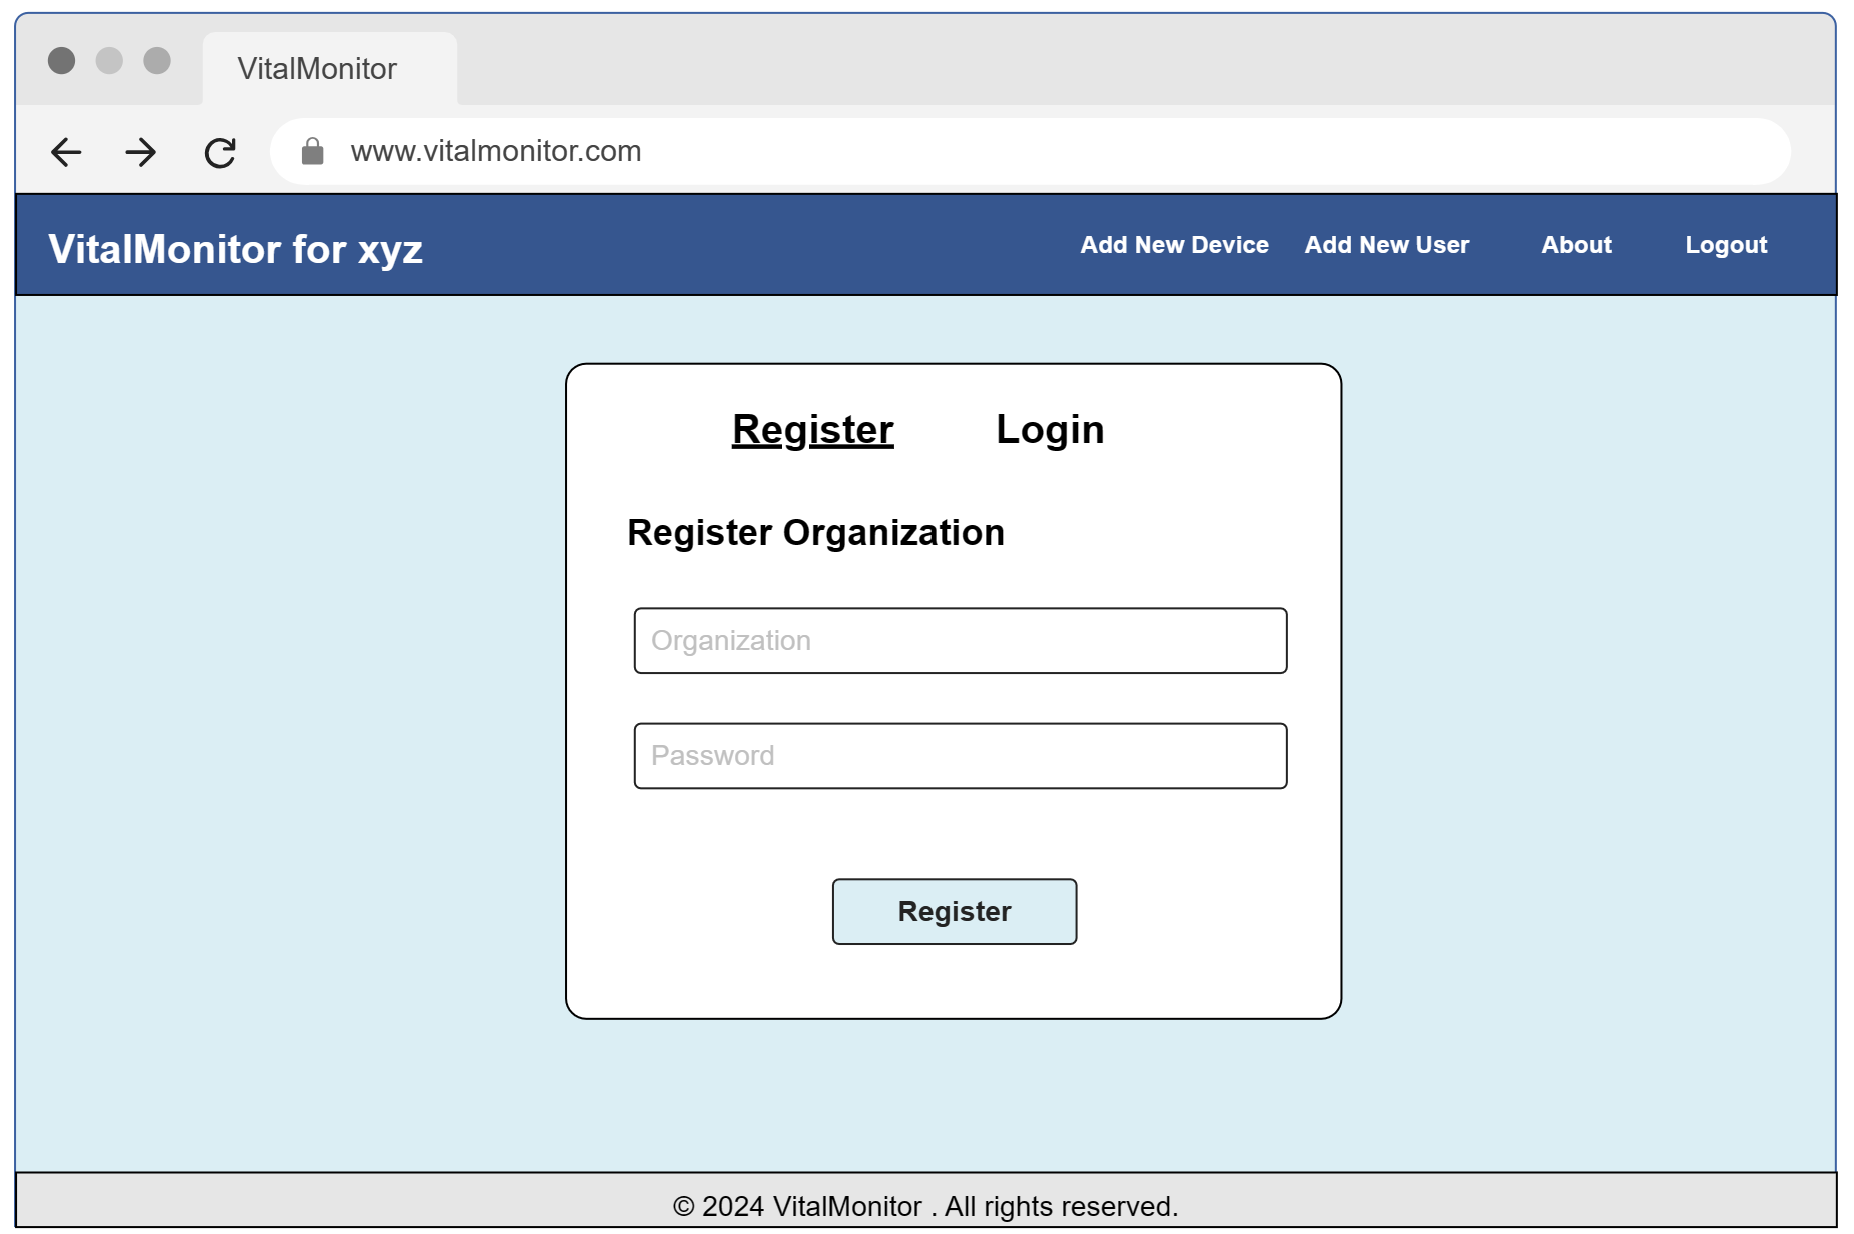
\includegraphics[width=0.87\linewidth]{images/register organization.png}
    \caption{Landing Page to register/login}
    \label{fig:wf-4}
\end{figure}

\begin{figure}[!h]
    \centering
    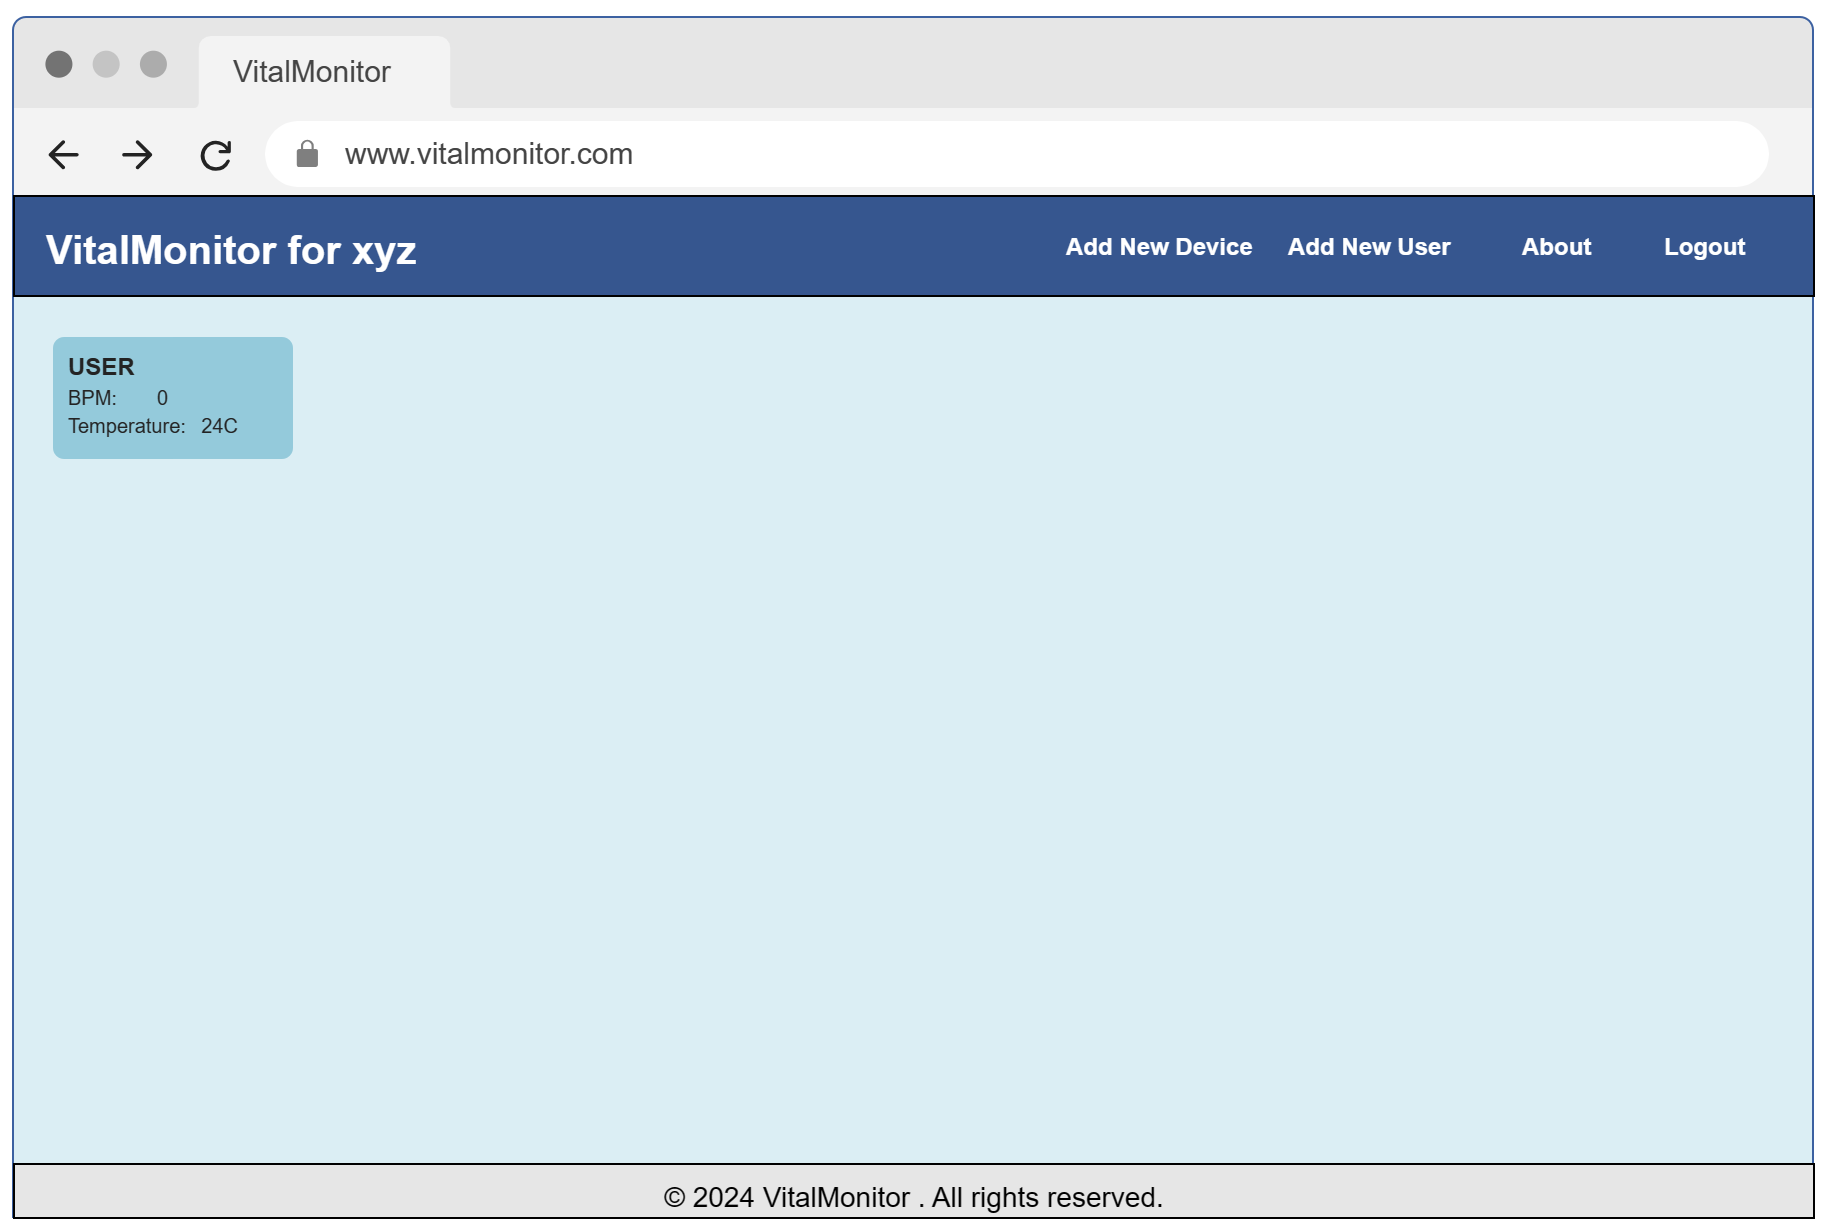
\includegraphics[width=0.87\linewidth]{images/home.png}
    \caption{Home Page}
    \label{fig:wf-3}
\end{figure}

\begin{figure}[!h]
    \centering
    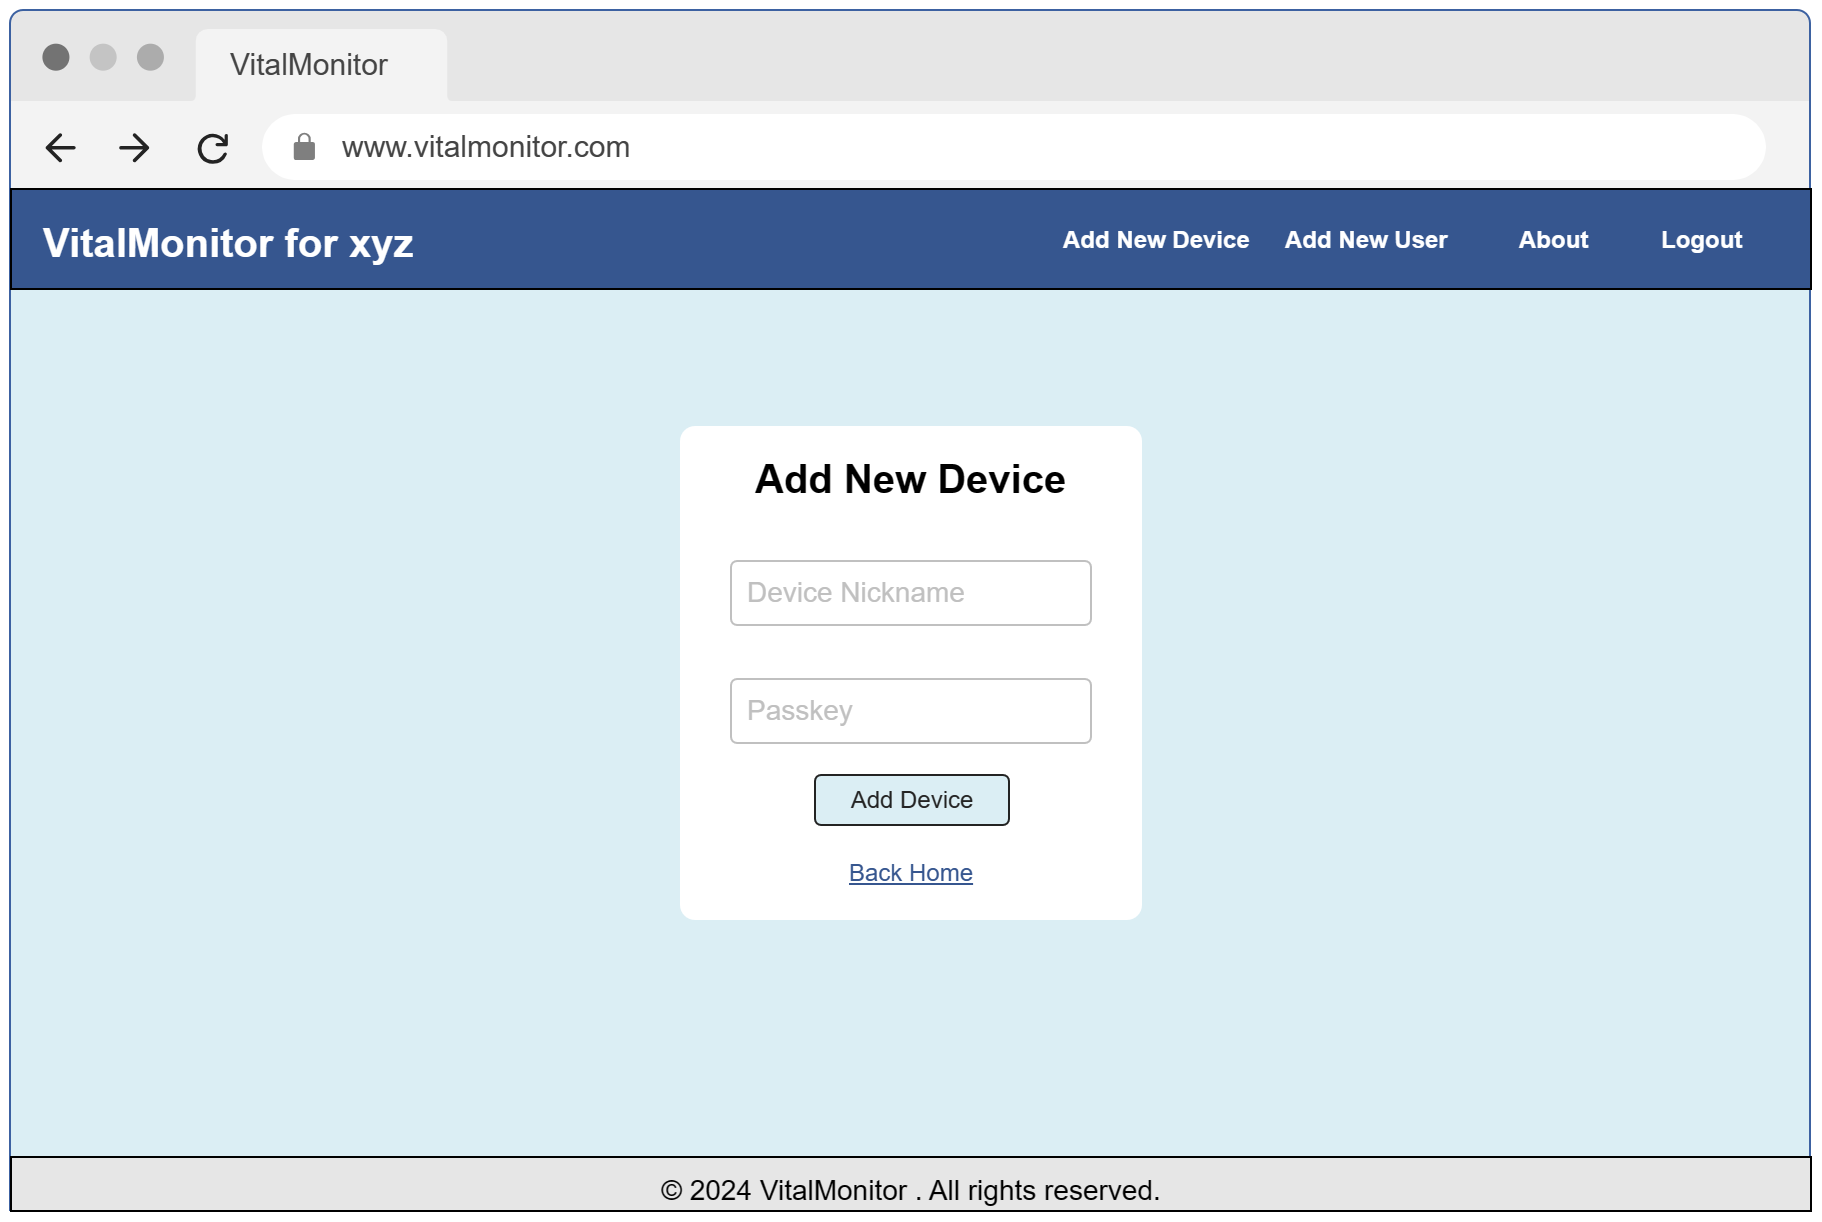
\includegraphics[width=0.9\linewidth]{images/Addnewdevice.png}
    \caption{Add New Device page}
    \label{fig:wf-1}
\end{figure}
\begin{figure}[!h]
    \centering
    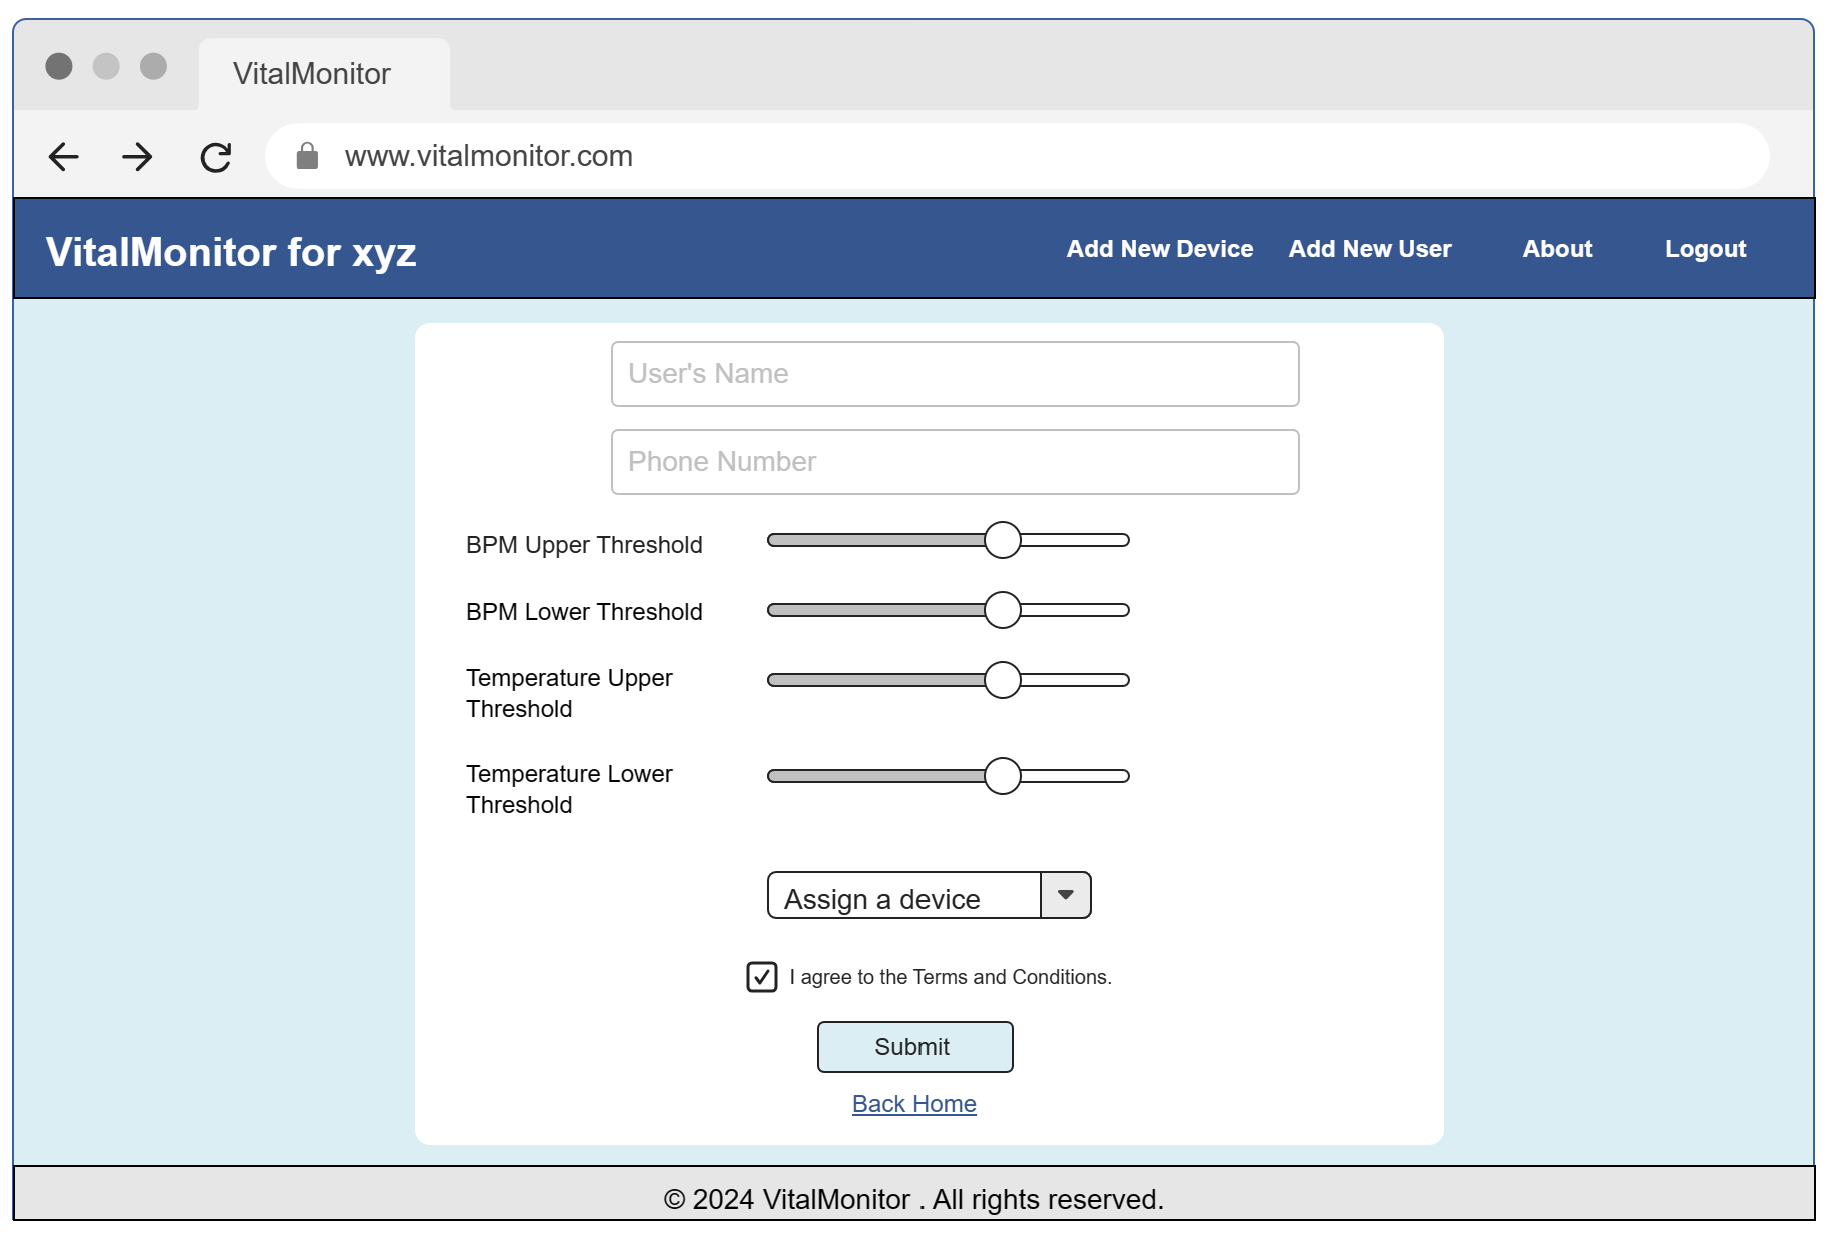
\includegraphics[width=0.9\linewidth]{images/addnewuser.png}
    \caption{Add New User Page}
    \label{fig:wf-2}
\end{figure}

\begin{figure}[!h]
    \centering
    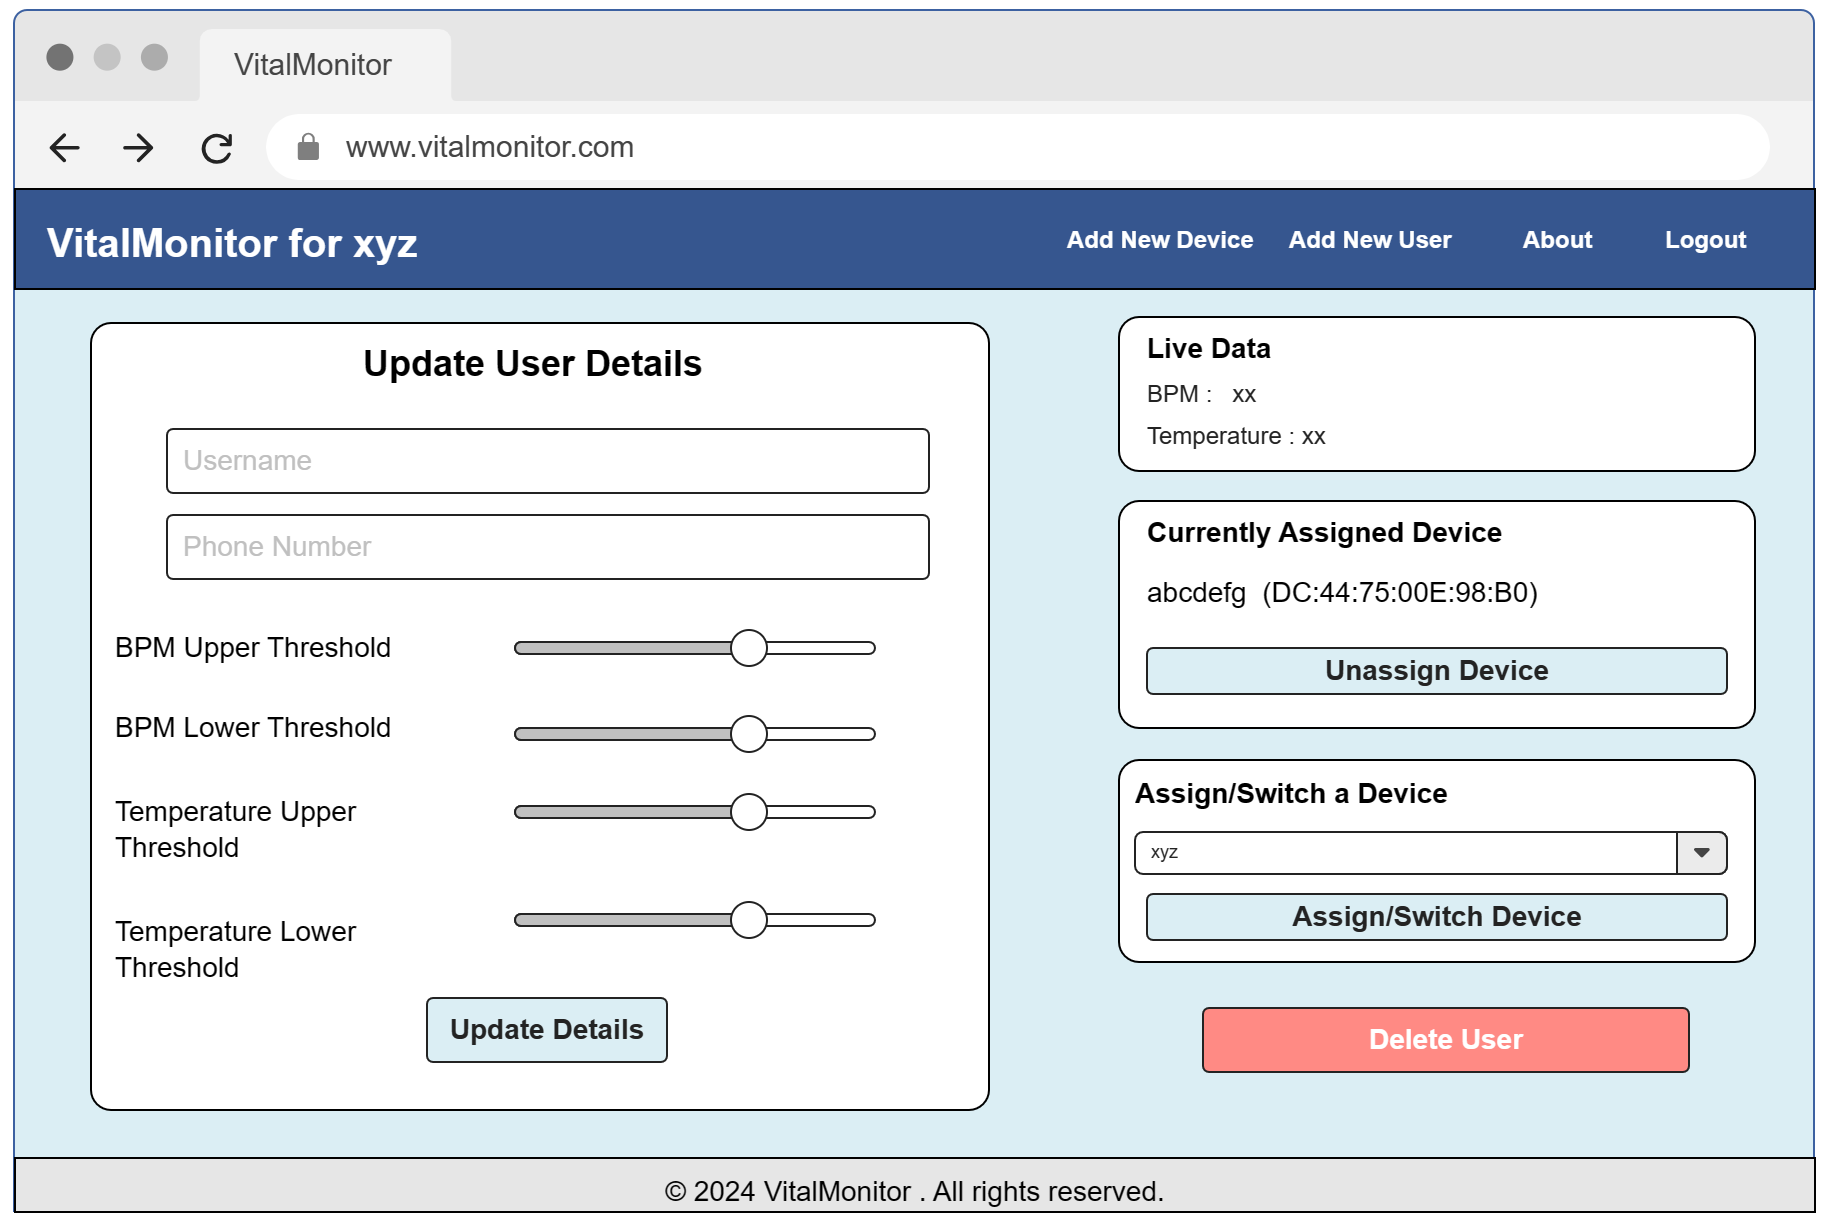
\includegraphics[width=0.9\linewidth]{images/update user details.png}
    \caption{User Page}
    \label{fig:wf-5}
\end{figure}
\begin{figure}[!h]
    \centering
    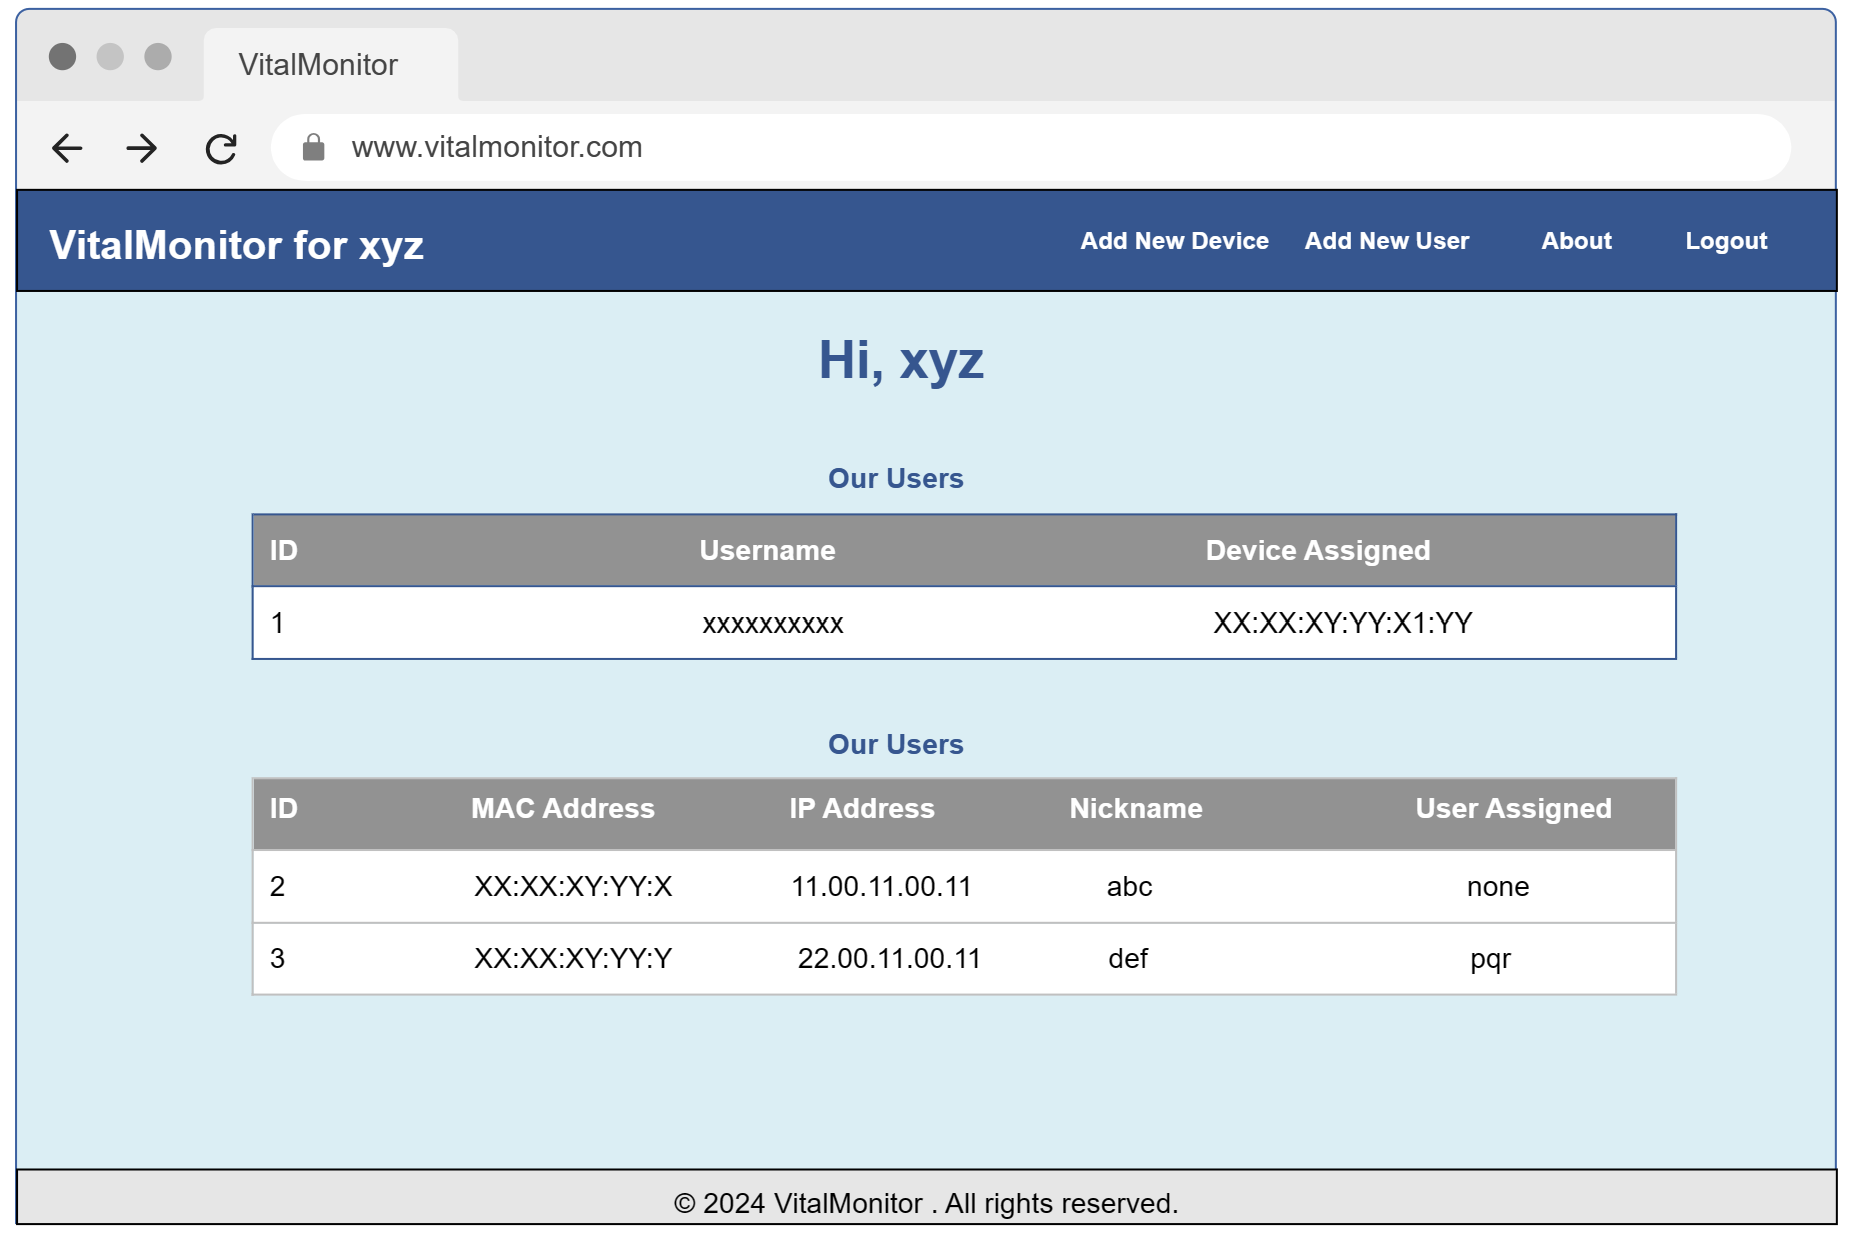
\includegraphics[width=0.9\linewidth]{images/VitalMonitor.png}
    \caption{About Page}
    \label{fig:wf6}
\end{figure}


\section{Network Communication and API Design}
VitalMonitor's networking layer is designed to enable robust and efficient interactions between front-end applications, back-end services, and IoT devices. By utilizing RESTful principles and leveraging the JSON data format, the system ensures streamlined data exchange and functionality that scales effectively with the demands of healthcare monitoring. Along with it, Smart Patches are designed to create their own Asyncronous Web Servers to facilitate transmission of data. Additionally, they are designed to use MQTT Protocol to publish data on Adafruit IO Dashboard.\\

\subsection{API and API Endpoints}
The API endpoints of VitalMonitor are meticulously designed to reflect a resource-oriented approach, enabling straightforward CRUD operations. Here’s a closer look at the design:

\begin{itemize}
    \item Structured for Simplicity and Efficiency: Each endpoint is crafted to represent and manipulate a distinct entity, such as users or devices, simplifying interactions and reducing complexity.
    \item Consistent Data Format: The system exclusively use JSON for all exchanges, ensuring compatibility and ease of development across various platforms.
    \item Stateless Operations: Ensuring each request is self-contained,  the APIs maintains statelessness, which is key to enhancing the scalability and reliability of distributed systems.
\end{itemize}

There are multiple API endpoints for each of the components of the system :\\

\subsubsection{Middleware:}
\begin{longtable}{|p{5cm}|p{1.5cm}|p{7.5cm}|}
\caption{API Endpoints for Middleware} \label{tab:api_endpoints} \\
\hline
\textbf{Endpoint} & \textbf{Method} & \textbf{Description} \\ \hline
\endfirsthead
\multicolumn{3}{c}%
{\tablename\ \thetable\ -- \textit{Continued from previous page}} \\
\hline
\textbf{Endpoint} & \textbf{Method} & \textbf{Description} \\ \hline
\endhead
\hline \multicolumn{3}{r}{\textit{Continued on next page}} \\
\endfoot
\hline
\endlastfoot

/register & POST & Register a new organization with name and password. \\ \hline
/login & POST & Authenticate organization credentials. \\ \hline
/add-new-user & POST & Add a new user to an organization, specifying necessary personal and health threshold details. \\ \hline
/add-new-device & POST & Add or update a device in the system, specifying details like MAC address and IP address. \\ \hline
/associate-device & POST & Associate a device with an organization using device nickname and passkey. \\ \hline
/assign-device-to-user & POST & Assign a device to a specific user, linking it with user ID and device ID. \\ \hline
/unassign-device/\{device\_id\}/\{user\_id\} & POST & Unassign a device from a user, removing all associated user details from the device. \\ \hline
/update-user-details & POST & Update details for an existing user, including contact information and health thresholds. \\ \hline
/get-device-data/\{device\_id\} & GET & Stream real-time data from a specific device. \\ \hline
/save-device-data & POST & Save data received from a device to the database. \\ \hline
/delete-device/\{device\_id\} & DELETE & Remove a device and all its associated data from the system. \\ \hline
/delete-user/\{user\_id\} & DELETE & Remove a user and all their associated details from the system. \\ \hline
/delete-organization/\{organization\_id\} & DELETE & Remove an entire organization and all associated users, devices, and data. \\ \hline
/devices & GET & Retrieve all devices associated with an organization. \\ \hline
/users & GET & Retrieve all users within an organization. \\ \hline
/user/\{user\_id\} & GET & Retrieve detailed information about a specific user. \\ \hline
\end{longtable}

\subsubsection{Dashboard:}
\begin{longtable}{|p{5cm}|p{1.5cm}|p{7.5cm}|}
\caption{Dashboard API Endpoints} \label{tab:dashboard_api_endpoints} \\
\hline
\textbf{Endpoint} & \textbf{Method} & \textbf{Description} \\ \hline
\endfirsthead
\multicolumn{3}{c}%
{\tablename\ \thetable\ -- \textit{Continued from previous page}} \\
\hline
\textbf{Endpoint} & \textbf{Method} & \textbf{Description} \\ \hline
\endhead
\hline \multicolumn{3}{r}{\textit{Continued on next page}} \\
\endfoot
\hline
\endlastfoot

/register & POST & Registers and logs in a new organization. \\ \hline
/login & POST & Authenticates and sets session for an organization. \\ \hline
/ & GET & Displays the main dashboard if logged in. \\ \hline
/register\_login & GET & Shows registration and login portal. \\ \hline
/logout & GET & Logs out and clears session. \\ \hline
/add-device-page & GET & Shows the add device page for logged-in users. \\ \hline
/add-device & POST & Adds a new device and displays status message. \\ \hline
/submit-user-details & GET & Displays unassigned devices for user assignment. \\ \hline
/add-user & POST & Adds a new user and optionally assigns a device. \\ \hline
/user/{user\_id} & GET, POST & Allows updating user details and device assignment. \\ \hline
/device/{device\_id}/update-details & POST & Sends updated user data to a device. \\ \hline
/sendDetails & POST & Receives and updates live BPM and temperature data. \\ \hline
/data-stream & GET & Streams live BPM and temperature data. \\ \hline
/about-us & GET & Displays organization details for logged-in users. \\ \hline
\end{longtable}


\subsubsection{Smart Patch:}
\begin{longtable}{|p{5cm}|p{1.5cm}|p{7.5cm}|}
\caption{Smart Patch API Endpoints} \label{tab:smart_patch_api_endpoints} \\
\hline
\textbf{Endpoint} & \textbf{Method} & \textbf{Description} \\ \hline
\endfirsthead
\multicolumn{3}{c}%
{\tablename\ \thetable\ -- \textit{Continued from previous page}} \\
\hline
\textbf{Endpoint} & \textbf{Method} & \textbf{Description} \\ \hline
\endhead
\hline \multicolumn{3}{r}{\textit{Continued on next page}} \\
\endfoot
\hline
\endlastfoot

/receive-user-details & POST & Receives and stores user details for device assignment, enabling personalized data monitoring and alerts. \\ \hline
/clear-user-details & POST & Clears all user-specific details from the device, effectively unassigning it from a user. \\ \hline
/stop-publishing & GET & Handles request to stop data publishing, which could be triggered remotely via web request. \\ \hline

\end{longtable}

Lastly, feeds will be designed as per MQTT Protocol for sending data to Adafruit IO Dashboard. See Appendix \ref{app:adafruit} for more information.

\newpage
\subsection{Error Handling and Management}
The implemented networking layer should be able to handle different HTTP client and server errors that can occur. The supported errors are: \\

\begin{table}[!h]
\centering
\begin{tabularx}{\textwidth}{|X|X|}
\hline
\textbf{Error Code} & \textbf{Error Descriptions}  \\ \hline
400 & Bad Request \\ \hline
401 & Unauthorised \\ \hline
404 & Not Found \\ \hline
409 & Conflict with current state/resources \\ \hline
500 & Network Errors  \\ \hline
\end{tabularx}
\caption{Supported Error Codes}
\label{tab:error-codes}
\end{table} 

More error conditions can be added in future, if deemed necessary. However, these cover the minimum needed to provide a reliable user experience.


